%In this stage we explain formally our modeling process of a benchmark to be solved (or study) through \posl{}. We explain how to make use of the already existing models or to create new benchmarks using the basic layer of the framework in C++ making a proper usage of the object-oriented design.

Target problems are modeled in \posl{} using the C++ programing language, respecting some rules of the object-oriented design. First of all, the benchmark must inherit from the \pclass{Benchmark} class provided by \posl. This class does not have any method to be overridden or implemented, but receives in its constructor three objects, instances of classes the user must create. Those classes must inherit from \pclass{SolutionCostStrategy}, \pclass{RelativeCostStrategy} and \pclass{ShowStrategy}, respectively. In these classes the most important functionalities of the benchmark model are defined.

\underline{\textbf{SolutionCostStrategy}}: In this class the strategy computing the \textit{cost} of a configuration is implemented. This \textit{cost function} must return an integer taking into account the problem constraints. Given a configuration $s$, the \textit{cost function}, as a mandatory rule, must return 0 if and only if $s$ is a solution of the problem, i.e., $s$ fulfills all the problem constraints. Otherwise, it must return an integer describing "how long" is the given configuration from a solution. An example of \textit{cost function} is the one returning the number of violated constraints. However, the more expressive the cost function is, the better the performance of \posl{} is, leading to the solution.

\poslexample{
Let us take the example of the {\it 4-Queens Problem}. This problem is about placing 4 queens on a $4\times 4$ chess board so that none of them can hit any other in one move. A configuration for this benchmark is a vector of 4 integer indicating the row where a queens is placed on each column. So, the configuration $s_a = (1,3,1,2)$ corresponds to the example in Figure~\ref{subqueen:1}. 

Now, let us suppose two different \textit{cost functions}:

\begin{enumerate}
\item $f_1(s) = c$ if and only if $c$ is the maximum number of queens hitting another.
\item $f_2(s) = c$ if and only if $c$ is the sum of the number of queens that each queen hits.
\end{enumerate}

Tacking these two functions into account, it is easy to see that $f_1(s_a) = 3$ and $f_2(s_a) = 4$. If we take the example in Figure~\ref{subqueen:2}, the corresponding configuration is $s_b = (0,1,0,2)$ with $f_1(s_b) = 3$ and $f_2(s_b) = 6$. In this case, according to the \textit{cost function} $f_1$ both configurations have the same opportunity of being selected, because they have the same cost. However, applying the \textit{cost function} $f_2$, the best configuration is $s_b$ in which a solution can be obtained just moving the queen \textit{b3} to \textit{a3}.

In that sense, $f_2$ is \textit{more expressive} than $f_1$.
}

\begin{figure}[h]
	\centering
	\subfloat[][]{
		\label{subqueen:1}
		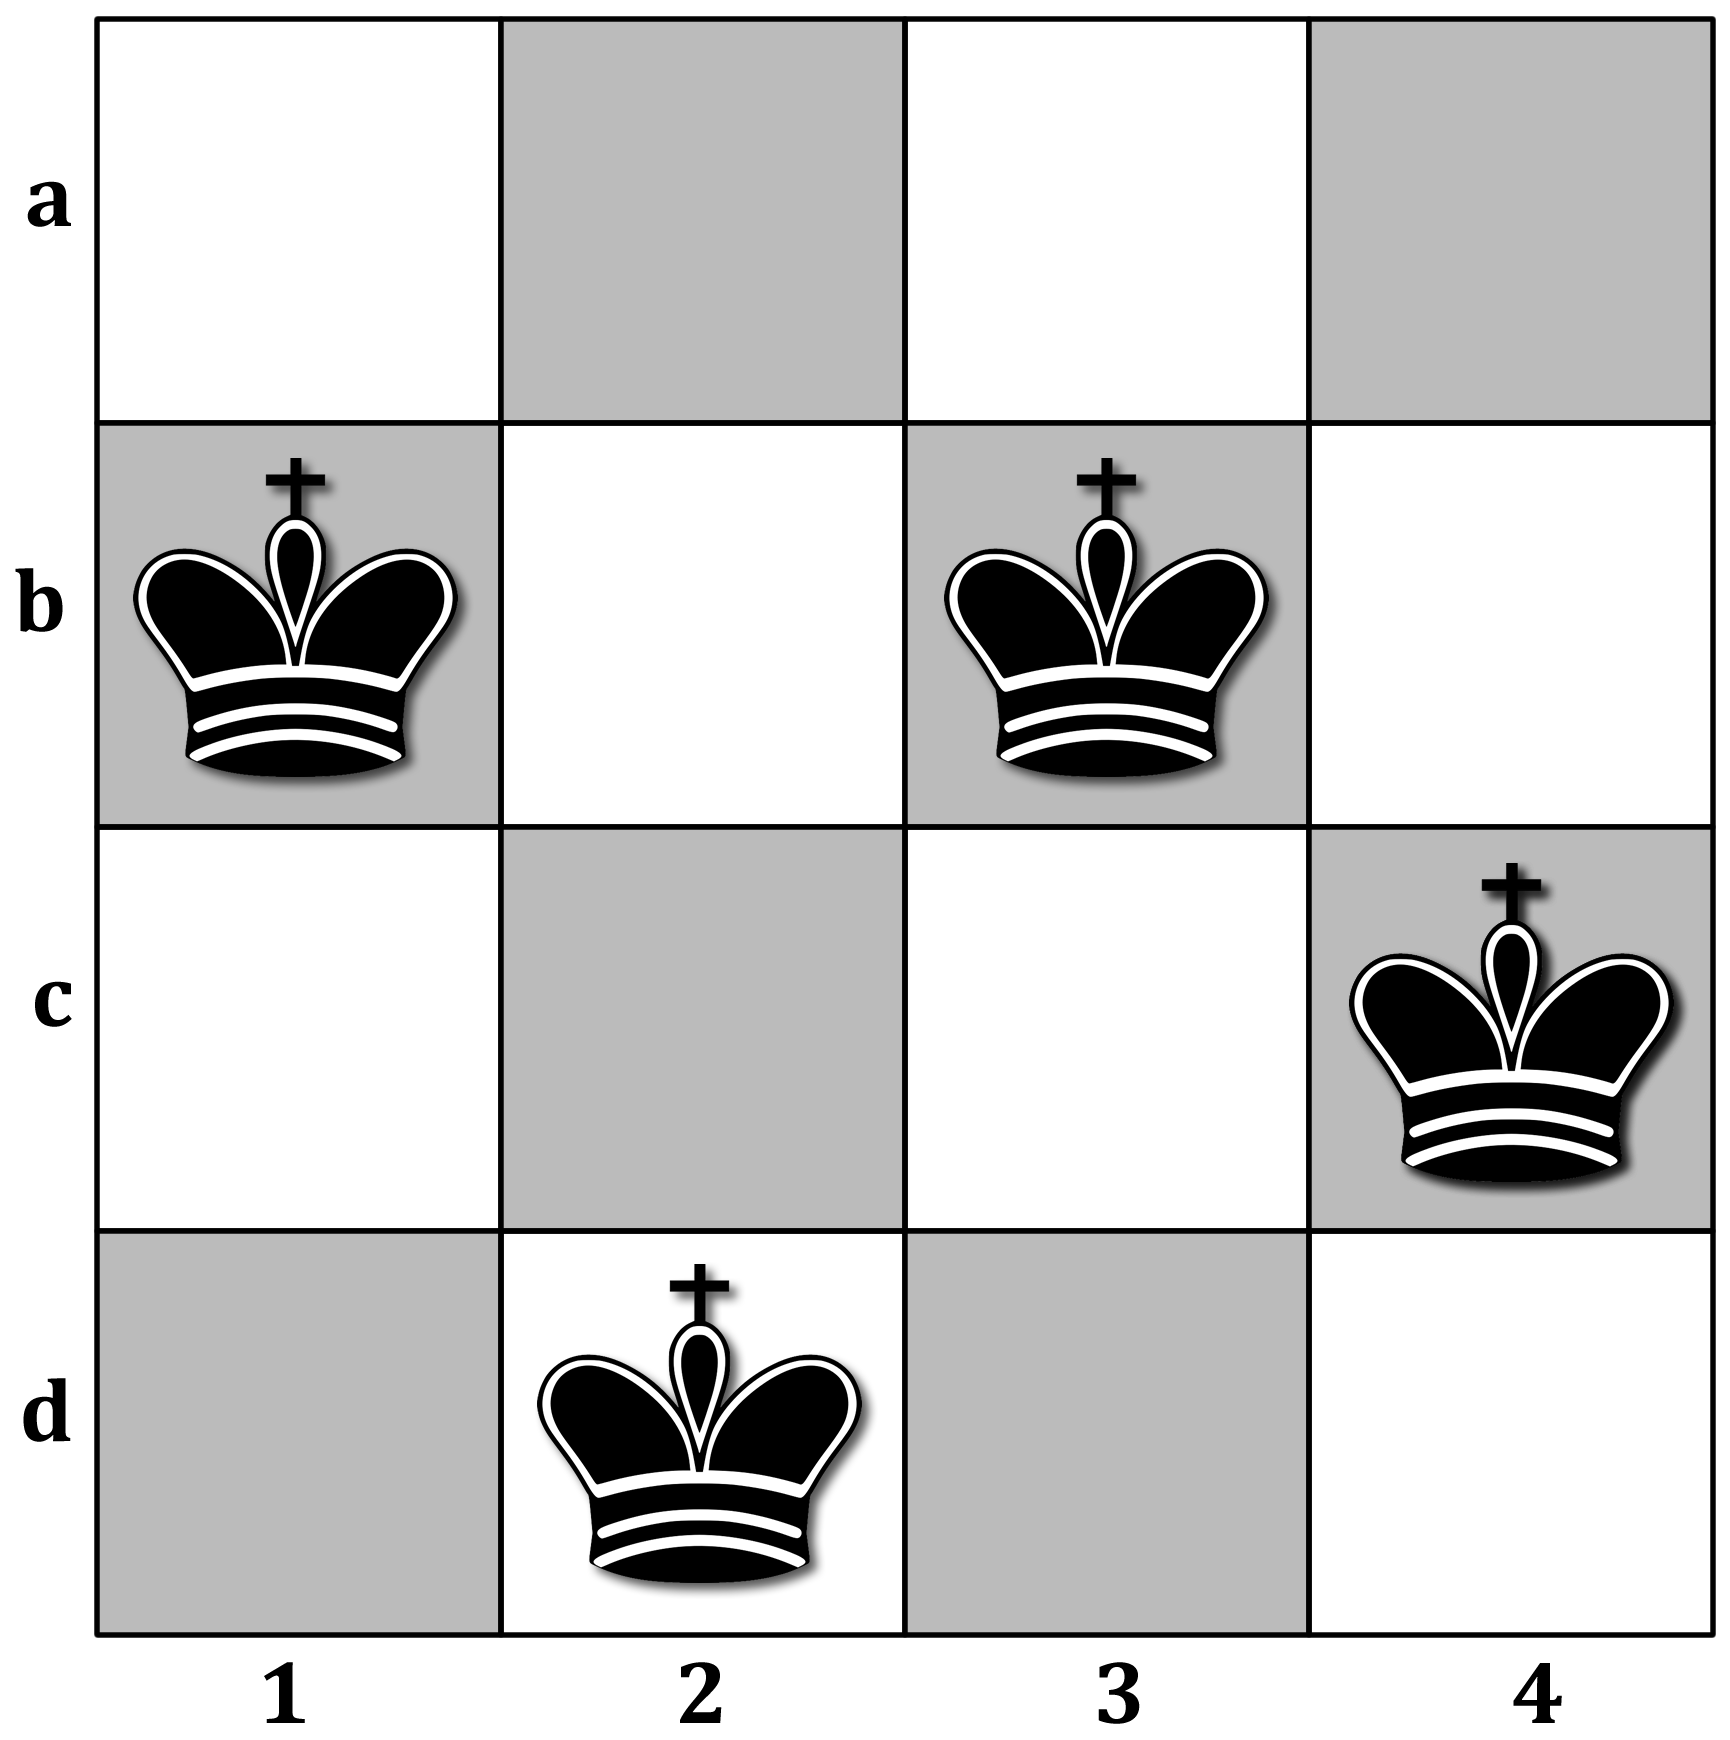
\includegraphics[width=0.25\linewidth]{queen1_1.png}
	}
	\hspace{0.05\textwidth}%
	\subfloat[][]{%
		\label{subqueen:2}
		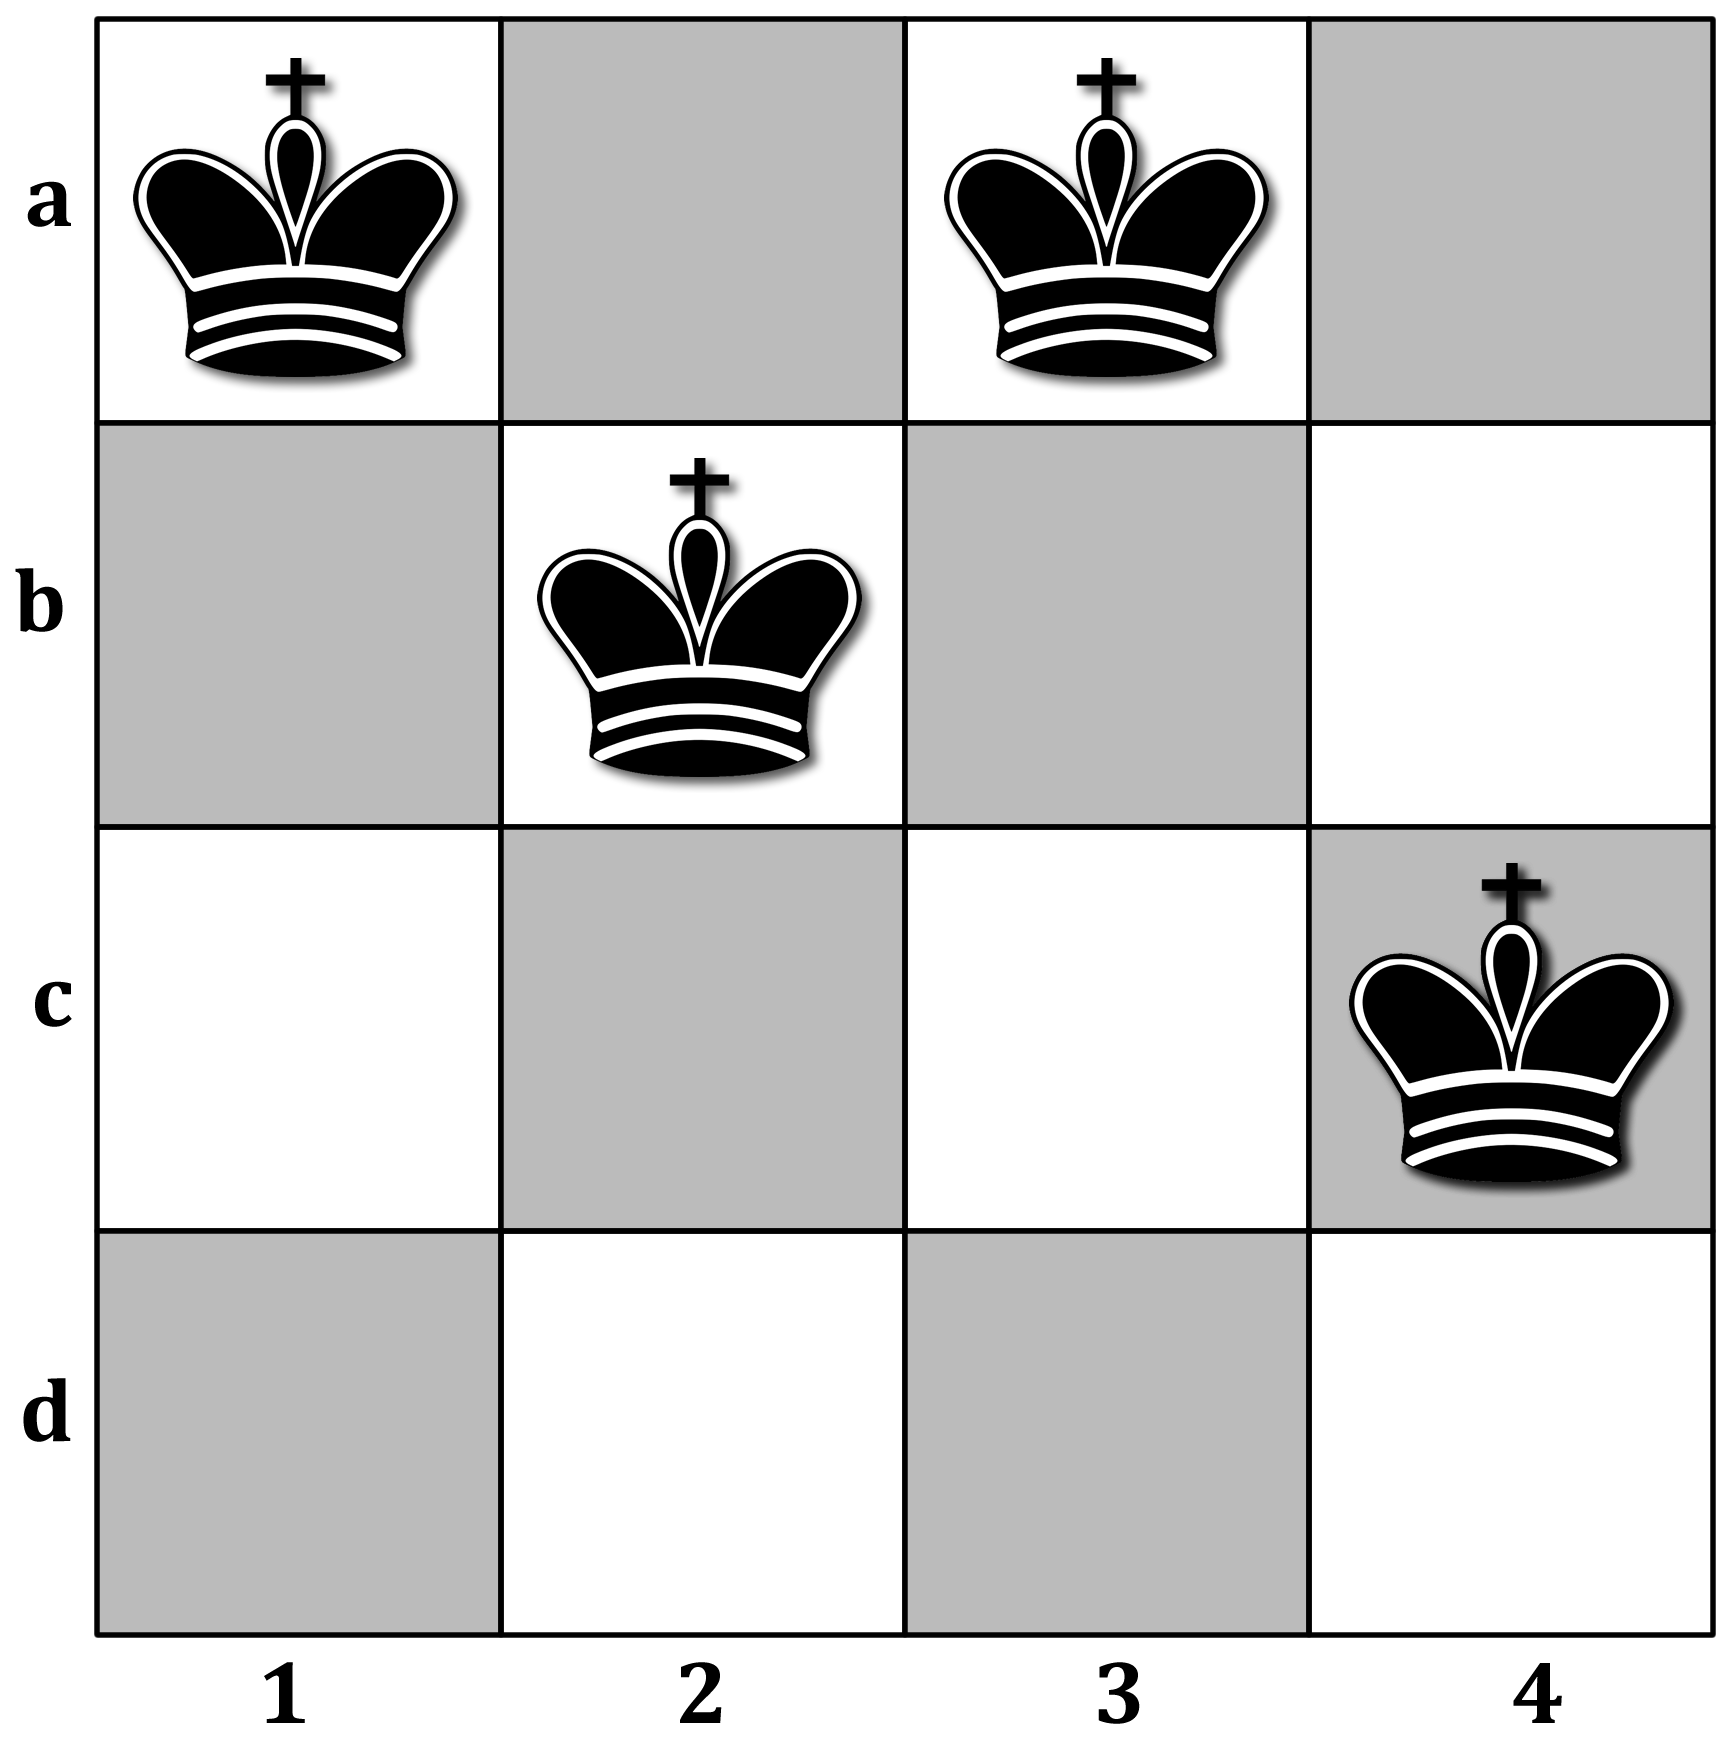
\includegraphics[width=0.25\linewidth]{queen1_2.png}
	}
	\hspace{0.05\textwidth}%
	\subfloat[][]{%
		\label{subqueen:3}
		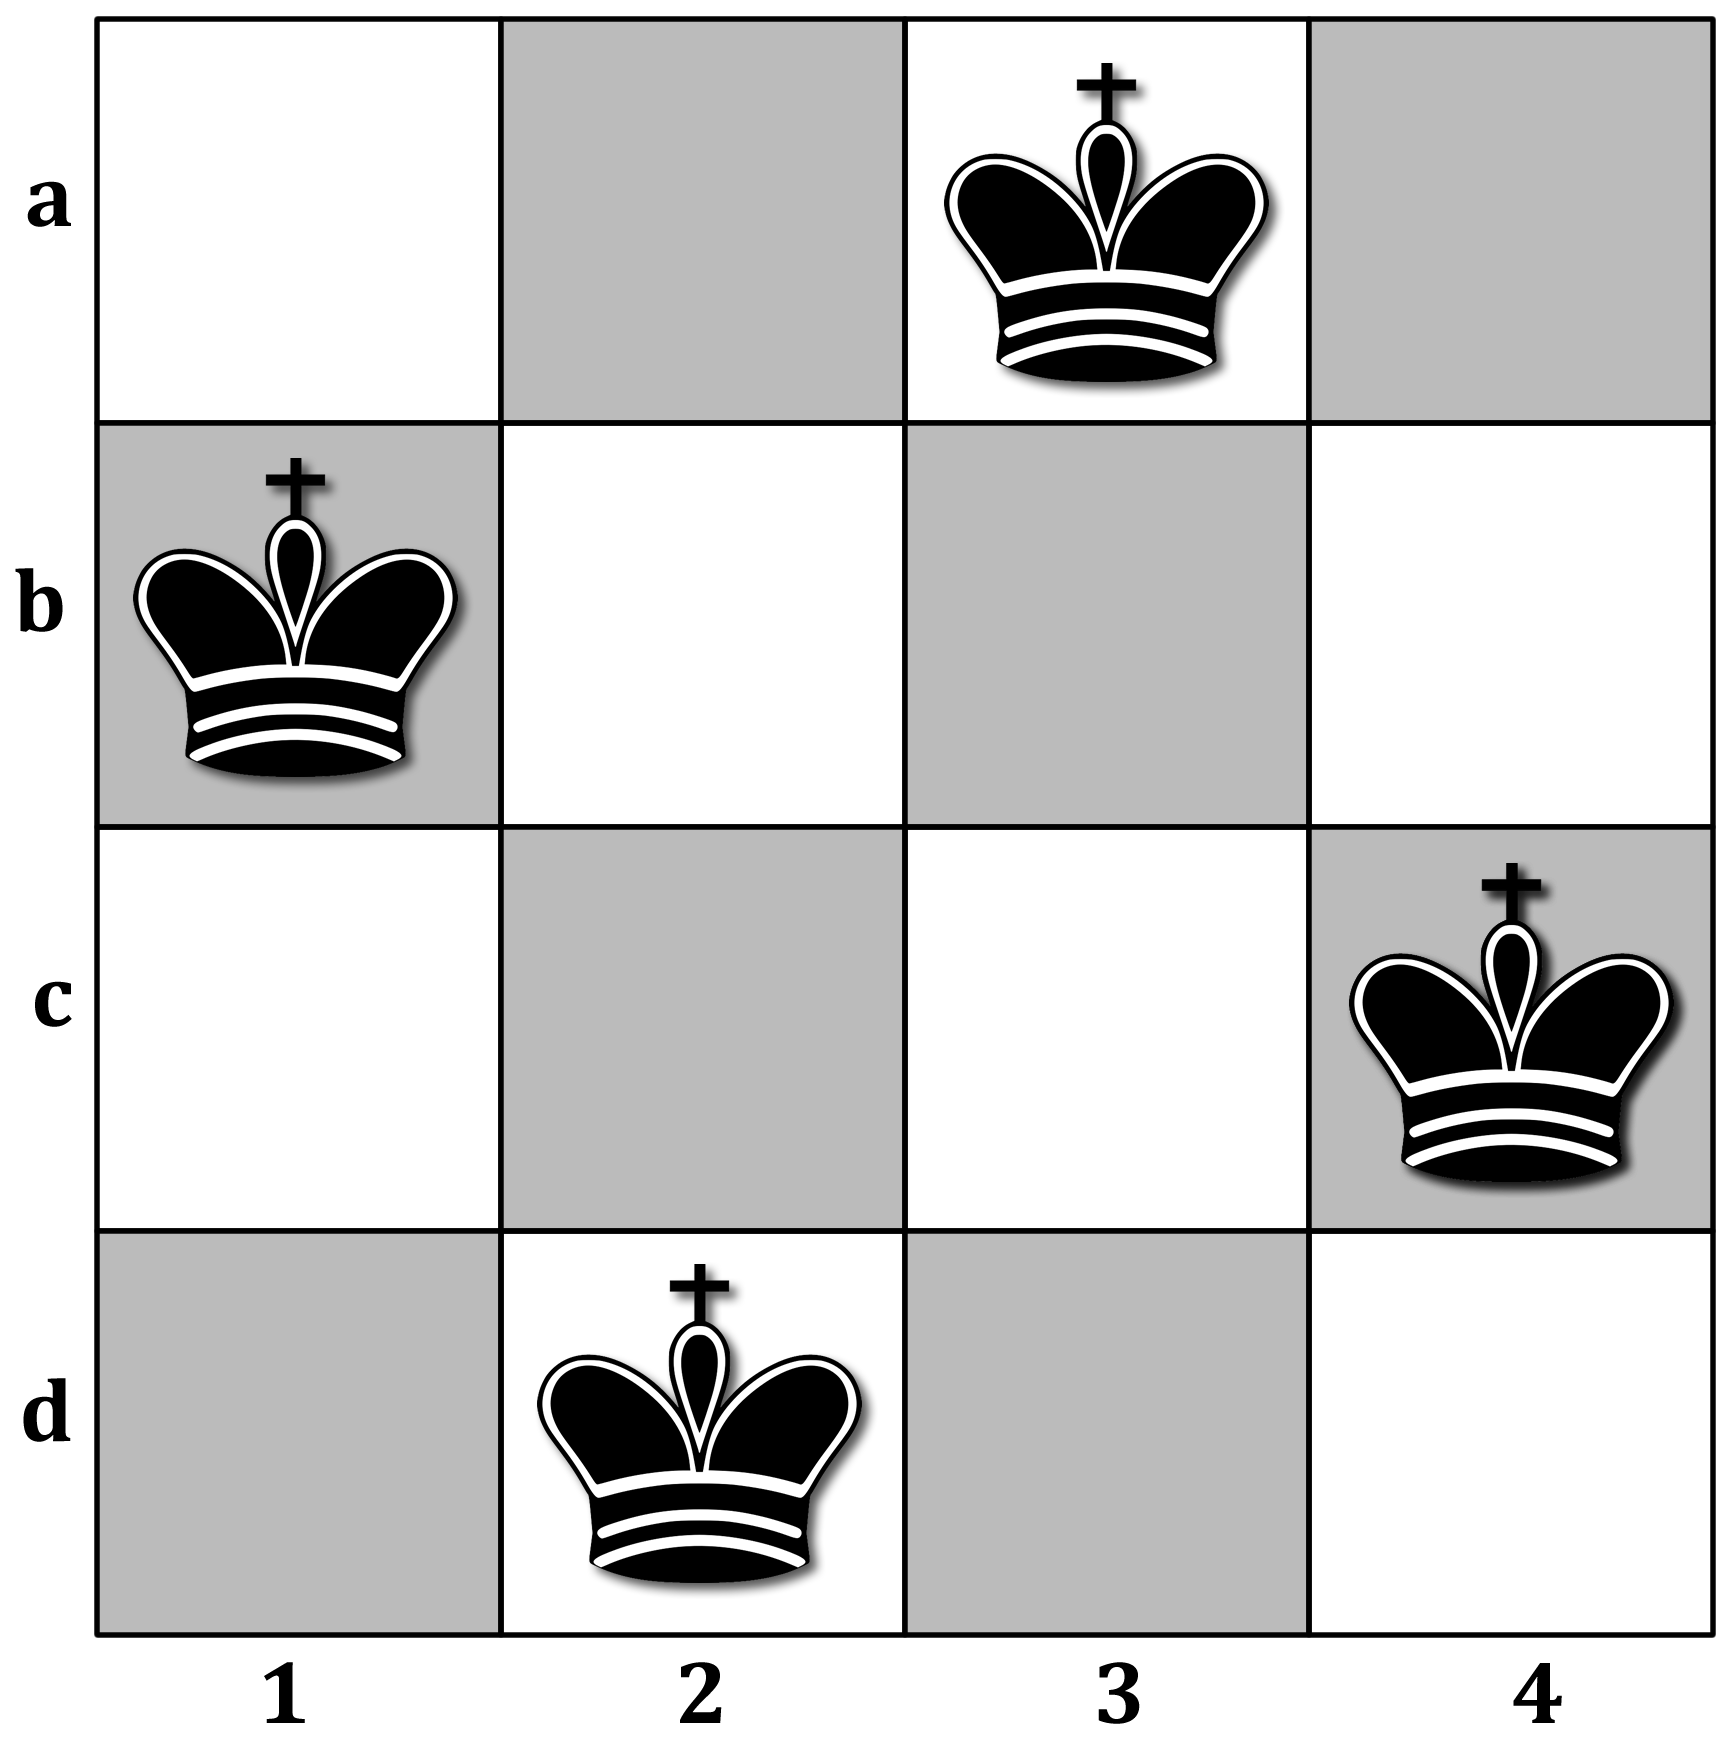
\includegraphics[width=0.25\linewidth]{queen1_3.png}
	}
	\caption[]{4-Queens examples}
	\label{fig:exqueens}
\end{figure}

The method to be implemented in this class is:

\begin{itemize}
\item \verb!int solutionCost(std::vector<int> & c)! $\rightarrow$ Computes the cost of a given configuration \verb!c!.
\end{itemize}

\underline{\textbf{RelativeCostStrategy}}: In this class the user implements the strategy to compute the \textit{cost} of a given configuration with respect to another, with the help of some stored information.

\poslexample{
Coming back to the previews example, let us suppose that the current configuration is $s_a = (1,3,1,2)$ corresponding to the Figure~\ref{subqueen:1}. Taking the \textit{cost function} $f_2$, the cost of this configurations is $f_2(s_a) = 4$. If we want to compute the cost of $s_c = (1, 3, 0, 2)$ (Figure~\ref{subqueen:3}), knowing that the only change with respect to the current configuration is the queen in the column $3$, we can use the following \textit{relative cost function}:
\begin{align*} 
rf(s_c) &=  c - 2\cdot q + a\\ 
&= 4 - 2\cdot 2 + 0 \\
&= 0
\end{align*}
where $c$ is the current cost, $q$ is the number of queens that the queen in column $3$ hits (an information that can be stored), and $a$ the number of queens that the queen in the column $3$ hits in the new position (\textit{a3}).
}

The methods to implement in this class are:

\begin{itemize}
\item \verb!void initializeCostData(std::vector<int> & c)! $\rightarrow$ Initializes the information related to the cost (auxiliary data structures, the current configuration \verb!c!, the current cost, etc.)
\item \verb!void updateConfiguration(std::vector<int> & c)! $\rightarrow$ Updates the information related to the cost.
\item \verb!int relativeSolutionCost(std::vector<int> & c)! $\rightarrow$ Returns the relative cost of the configuration \verb!c! with respect to the current configuration.
\item \verb!int currentCost()! $\rightarrow$ Property that returns the cost of the current configuration.
\item \verb!int costOnVariable(int variable_index)! $\rightarrow$ Returns a measure of the contribution of a variable to the total cost of a configuration. % \tet{AMPLIAR}
%\item \verb!int sickestVariable()! $\rightarrow$ Returns the variable contributing the most to the cost.
\end{itemize}

\underline{\textbf{ShowStrategy}}: This class represents the way a benchmark shows a configuration, in order to provide more information about the structure. 

%\poslexample{
For example, a configuration of the instance 3--3--2 of the \sgp{} (see bellow for more details about this benchmark) can be written as follows:

\begin{Verbatim}
[1, 2, 3, 4, 5, 6, 7, 8, 9, 3, 4, 5, 6, 7, 8, 9, 1, 2]
\end{Verbatim}

This text is, nevertheless, very difficult to be read if the instance is larger. Therefore, it is recommended that the user implements this class in order to give more details and to make it easier to interpret the configuration. For example, for the same instance of the problem, a solution could be presented as follows:

\begin{Verbatim}
Golfers: players-3, groups-3, weeks-2
6	8	7	
1	3	5	
4	9	2	
--
7	2	3	
4	8	1	
5	6	9	
--
\end{Verbatim}
%}

The method to be implemented in this class is:

\begin{itemize}
\item \verb!std::string showSolution(std::shared_ptr<Solution> s)! $\rightarrow$ Returns a string to be written in the standard output.
\end{itemize}

Once we have modeled the target benchmark, it can be solved using \posl{}. In the following sections we describe how to use this parallel-oriented language to solve \CSPs.